\chapter{User study} \label{chapter3}

Before designing the application, we needed to find out more about the needs and wants of students enrolled at \acrshort{acs}, as well as the general context in which this application would function.

\section{Methods} \label{3:methods}

The research and data collection methods we used were \textbf{observation} (throughout the four years that the main author of the paper was enrolled at our faculty of choice, \acrshort{acs}), \textbf{interviews} (with students, professors as well as administrative personnel of the faculty) and a \textbf{survey}, the results of which we will be focusing on in this chapter.  The results of the first two methods are mentioned and discussed throughout the whole paper, where offering insightful information for the specific section. Additionally, throughout every step of the whole process of designing the application, we went through a \textbf{feedback loop} with a small group of students to ensure that we were progressing in the right direction.

Partly due to the pandemic, the main method of communication with our potential users was online communication. Most of the interviews were done either via video call (through Microsoft Teams\footnote{https://teams.microsoft.com/}) or via chat (Facebook Messenger\footnote{https://messenger.com/}, WhatsApp\footnote{https://www.whatsapp.com/}) or e-mail (Gmail\footnote{http://gmail.com/}). The survey was a Google Form\footnote{http://forms.google.com/} shared both verbally and through social media platforms, receiving 212 responses between October and December 2019. Since we regrettably could not gather a relevant number of responses from Master's students, with only 7 responses, we will be focusing on the Bachelor's students, since a number of 200 out of the total of about 600 enrolled B.Sc. students is statistically relevant.

In order to analyze the data, we imported the results from the form into a database using Microsoft SQL Server\footnote{https://www.microsoft.com/en-us/sql-server/}, normalized the data and created visualizations using Microsoft Power BI\footnote{https://powerbi.microsoft.com/}.

\section{Target audience} \label{3:target_audience}

Studies\cite{hammer2011importance}\cite{connelly2013demographic} show that demographic information in surveys helps to avoid bias towards a specific section of the target audience, therefore we included some demographics questions to ensure that the pool of respondents is relatively balanced.

In terms of gender demographics, our results (fig. \ref{3:fig:gender}) closely match a separate study\cite{codette2019stats} that is specifically targeting gender demographics at computer science faculties in Romania, including \acrshort{acs}.

\begin{figure}[ht]
    \centering
         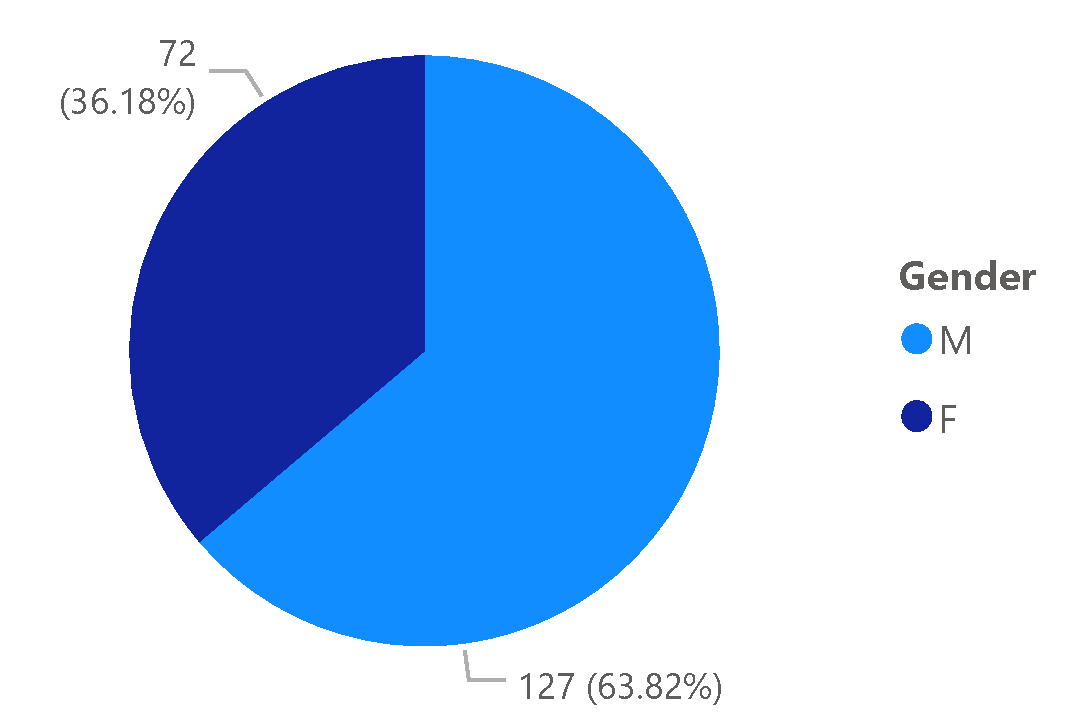
\includegraphics[height=0.2\textheight]{figures/charts/survey/gender.pdf}
    \caption{Gender of survey respondents}
    \label{3:fig:gender}
\end{figure}

Concerning university group distribution, we have received  four times more responses from students pursuing the Computer Science domain (Computers and Information Technology, or CTI) than the Automatics domain (Systems Engineering, or IS), as seen in figure \ref{3:fig:domain}. The distribution of the respondents' year of study is relatively balanced (fig. \ref{3:fig:year}).

\begin{figure}[!ht]
    \centering
    \begin{minipage}[b]{0.49\textwidth}
        \captionsetup{justification=centering}
         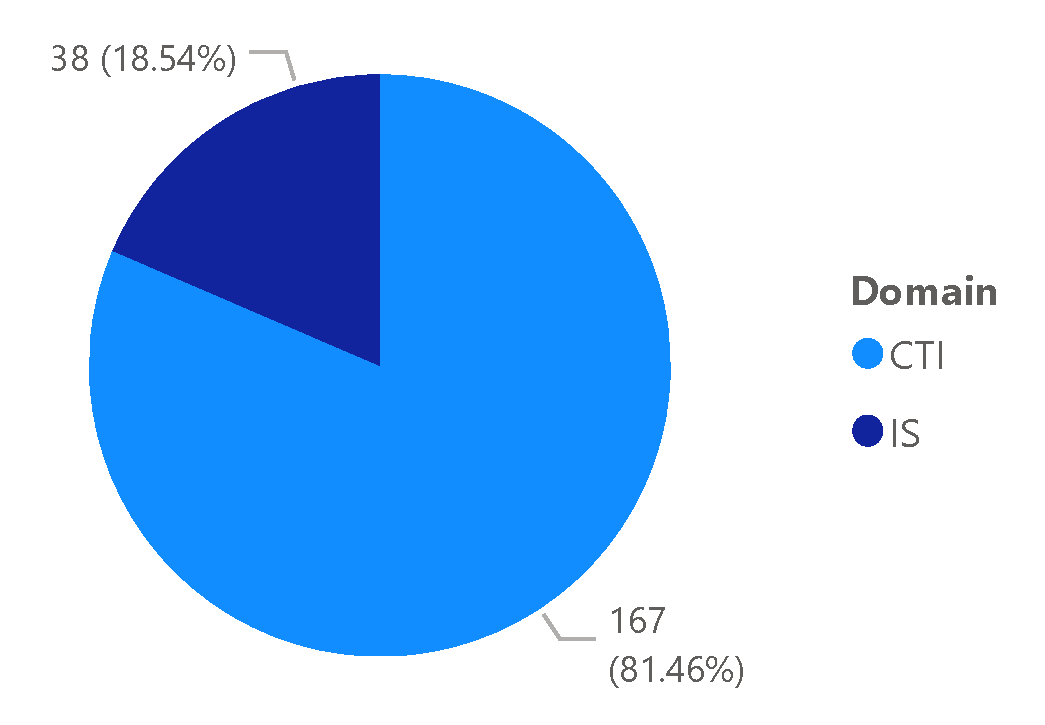
\includegraphics[height=0.2\textheight]{figures/charts/survey/domain.pdf}
        \caption{Domain of survey respondents}
        \label{3:fig:domain}
    \end{minipage}
    \hfill
    \begin{minipage}[b]{0.49\textwidth}
        \captionsetup{justification=centering}
         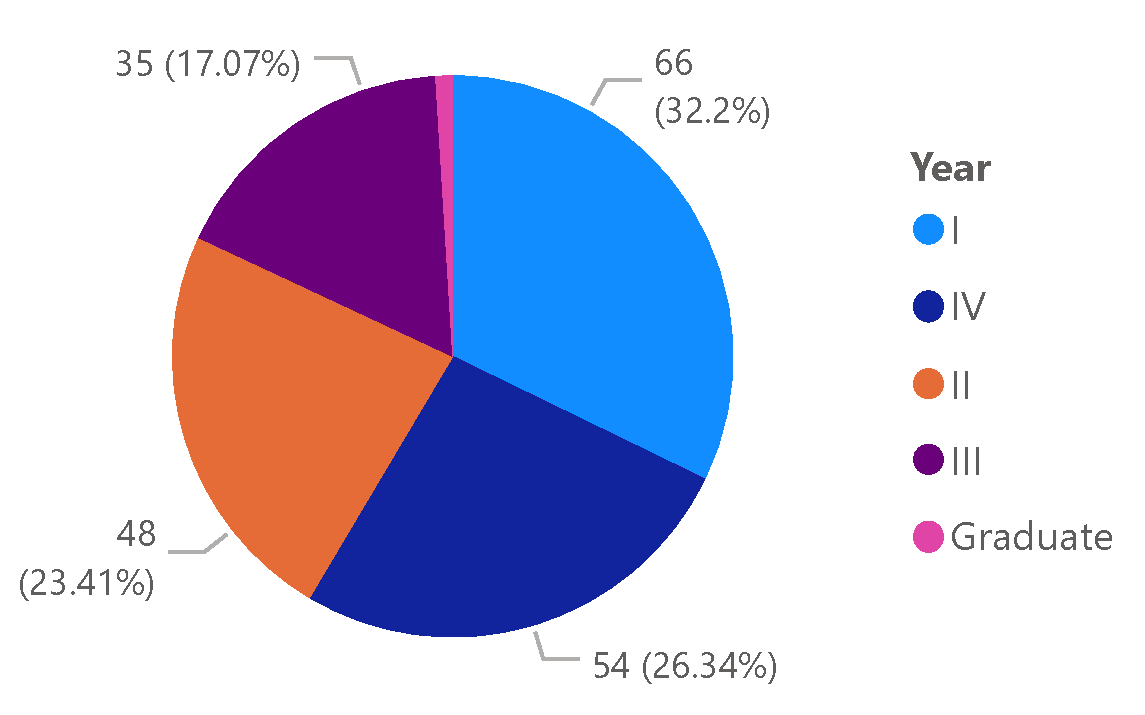
\includegraphics[height=0.2\textheight]{figures/charts/survey/year.pdf}
        \caption{Academic year of survey respondents}
        \label{3:fig:year}
    \end{minipage}
\end{figure}

Regarding mobile operating systems, the distibution is very similar to the Romanian mobile operating system market share according to StatCounter GlobalStats \cite{statcounter2020mobile}, with 80\% of students using Android and 20\% of students using iOS.

\begin{figure}[ht]
    \centering
         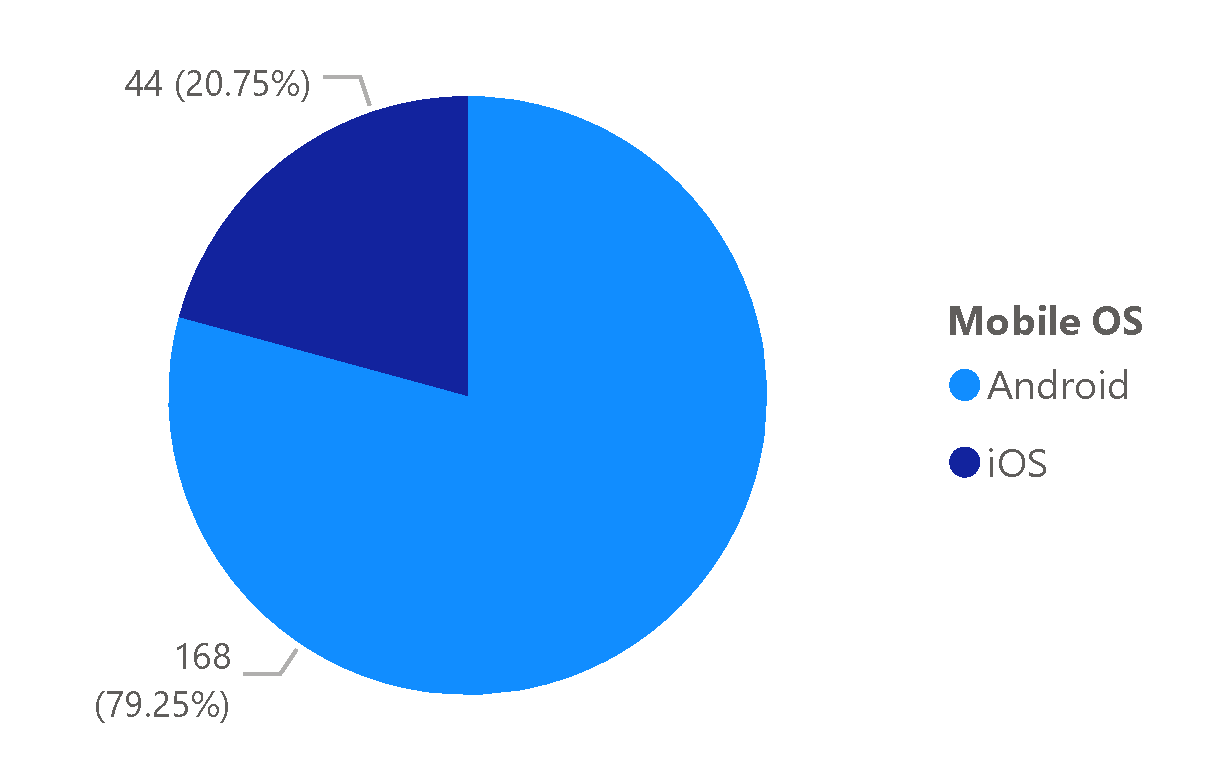
\includegraphics[height=0.2\textheight]{figures/charts/survey/os.pdf}
    \caption{Mobile \acrshort{os} of survey respondents}
    \label{3:fig:os}
\end{figure}

Upon reviewing the data, we believe that, aside from the lack of representation for Master's students, the respondents' demographics are varied enough to make for a relevant sample group.

\section{Results} \label{3:results}